\chapter{Teoria dei giochi} % (fold)
\label{cha:teoria_dei_giochi}
La teoria dei giochi analizza le decisioni individuali in situazioni in cui vi sono iterazioni tra agenti\footnote{un agente è un entità che partecipa al processo decisionale.} diversi, tali per cui le decisioni di un agente possono influire sui risultati conseguibili da parte dei rivali.\\

Queste situazioni conflittuali si possono vedere come dei \emph{giochi}, caratterizzati da tre componenti:
\begin{enumerate}
	\item \textbf{giocatori}: gli agenti che partecipano al conflitto;
	\item \textbf{strategie}: le possibili azioni o decisioni che ciascun agente può prendere;
	\item \textbf{utilità o payoff}: il beneficio che un giocatore ottiene nel adottare una certa strategia in un dato contesto di gioco\footnote{con contesto di gioco si intende l’insieme di strategie giocate da ciascun agente.}.
\end{enumerate}

\section{Giochi finiti in forma normale} % (fold)
\label{sec:giochi_finiti_in_forma_normale}

% section giochi_finiti_in_forma_normale (end)
Un gioco finito in forma normale consiste in un insieme di \emph{giocatori}
\begin{align}
	I= \{ 1,\dots, n\} (n \geq 2)
\end{align} ciascuno dei quali ha associato un insieme di strategie pure 
\begin{align}
	S_i = \{ 1, \dots, m_i \} \qquad m_i \geq 2
\end{align}
Una \textbf{strategia pura} fornisce una definizione completa del modo in cui un giocatore gioca una partita. In particolare, essa determina quale mossa farà il giocatore in qualsiasi situazione che potrebbe affrontare.
L’insieme delle strategie pure $s_i$ giocate dagli individui in un dato istante forma un \emph{profilo strategico} puro.
\begin{align}
	\mathbf{s} = (s_1, s_2, \dots, s_n)
\end{align}

\emph{Nota: i simboli in grassetto indicano un vettore.}

\newpage

L’insieme dei profili strategici puri forma lo \emph{spazio delle strategie} pure.
\begin{align}
	S = S_1 \times \cdots \times S_n
\end{align}

In seguito alla giocata di un profilo strategico $\mathbf{s} \in S$ ciascun individuo $i \in I$ ottiene un \emph{payoff}. Con il termine payoff si intende una quantificazione del beneficio che un individuo ha in seguito ad una giocata; in economia il payoff può denotare il profitto di un impresa o l’utilità di un consumatore. Ovviamente lo scopo di ogni giocatore è di massimizzare il payoff. \\

Si rappresenta il payoff dell’i-esimo giocatore come una funzione $\pi_i : S \rightarrow \R.$ La \emph{funzione di payoff combinata} $\pi : S \rightarrow \R_n$ assegna a ogni profilo strategico puro $\mathbf{s}$ il vettore di payoffs $\pi(\mathbf{s}) = (\pi_1(\mathbf{s}), \pi_2(\mathbf{s}), \dots , \pi_n(\mathbf{s}))$.\\

Nel caso speciale di giochi a due giocatori, è utile rappresentare le due funzioni di payoff in forma matriciale assegnando al primo giocatore la matrice di payoff 
\begin{align*}
	A = (a_{hk}) \qquad \text{dove } a_{hk} = \pi_1(h, k), \forall h,k \in S_1
\end{align*}
e al secondo giocatore la matrice 
\begin{align*}
	B = (b_{hk}) \qquad \text{dove } b_{hk} = \pi_2(h, k), \forall h,k \in S_2
\end{align*}
Ogni riga di ciascuna delle due matrici corrisponde quindi ad una strategia pura giocata dal giocatore 1, mentre ogni colonna corrisponde ad una strategia pura giocata dal giocatore 2.\\

È possibile a questo punto rappresentare un gioco in forma normale come una tripletta $G = (I, S, \pi)$ dove $I$ è l’insieme di individui, $S$ è lo spazio delle strategie pure e $\pi$ è la funzione di payoff combinata.\\

Si suppone ora che ciascun giocatore $i$ decida la strategia pura da usare in base ad una distribuzione di probabilità sull’insieme di strategie pure $S_i$. È possibile rappresentare questa distribuzione con un vettore $m_i$-dimensionale $\mathbf{x}_i$ nello spazio $\R^{m_i}$. La componente $x_{ih}$ rappresenterà la probabilità che la strategia pura $h$ sia usata dal giocatore $i$.\\

Si parla in questo caso di \textbf{strategia mista} per un giocatore; una distribuzione di probabilità sull'insieme delle strategie pure che costui ha a disposizione.

\newpage

Trattandosi di distribuzioni di probabilità si ottiene che ciascuna componente $x_{ih}$ con $h = {1,2,...}$ è positiva e la loro somma è uguale a 1, quindi il vettore appartiene al simplesso unitario $\Delta_i$ $m_i$-dimensionale.
\begin{align}
	\Delta_i = \left\{ x_i \in \R^{m_i}_+ : \forall h = 1, \dots, m_i : x_{ih} > 0 \text{ and } \sum_{h=1}^{m_i} x_{ih} = 1 \right\}
\end{align}
\begin{align*}
	\Delta_i = \left\{ x_i \in \R^{m_i}_+ : \mathbf{e}'\mathbf{x_i} = 1 \right\} \tag{Notazione vettoriale}
\end{align*}


\begin{figure}[h!]
	\centering
	\subfigure[]{
	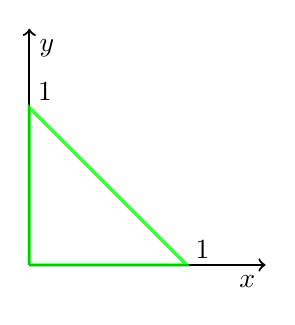
\begin{tikzpicture}[scale=2]
        %draw the main coordinate system axes
        \draw[thick,->] (0,0) -- (1.5,0) node[anchor=north east]{$x$};
        \draw[thick,->] (0,0) -- (0,1.5) node[anchor=north west]{$y$};
        
        \draw[thick, opacity=0.8, color=green, very thick] plot coordinates{(0,0) (0,1) (1,0) (0,0)};
    
        \node at (1.1,0.1) {1};
        \node at (0.1,1.1) {1};
    \end{tikzpicture}}
	\qquad\qquad
	\subfigure[]{
	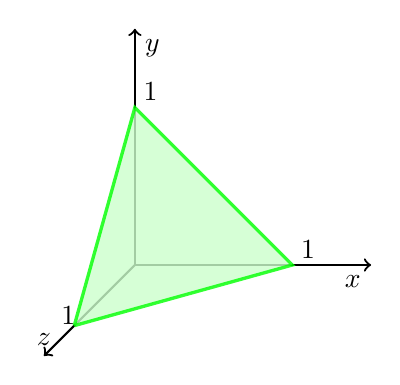
\begin{tikzpicture}[scale=2]
        %draw the main coordinate system axes
        \draw[thick,->] (0,0,0) -- (1.5,0,0) node[anchor=north east]{$x$};
        \draw[thick,->] (0,0,0) -- (0,1.5,0) node[anchor=north west]{$y$};
        \draw[thick,->] (0,0,0) -- (0,0,1.5) node[anchor=south]{$z$};
    
        \filldraw[thick, opacity=0.8, color=green!20, draw=green, very thick] plot coordinates{(0,0,1) (0,1,0) (1,0,0) (0,0,1)};
    
        \node at (1.1,0.1,0) {1};
        \node at (0.1,1.1,0) {1};
        \node at (0,0.1,1.1) {1};
	\end{tikzpicture}}
	\caption{A sinistra il simplesso a due dimensioni. A destra il simplesso a tre dimensioni. Da notare che le strategie pure corrispondono ai lati del simplesso standard.}
\end{figure}

L’insieme delle componenti di $\mathbf{x_i} \in \Delta_i$ a cui sono state assegnate probabilità non nulle forma il \emph{supporto} di $\mathbf{x_i}$
\begin{align*}
	\sigma(\mathbf{x_i}) = \{h \in S_i : x_{ih} > 0 \}
\end{align*}

Una strategia pura $h$ può essere vista come una strategia mista estrema $x_i$ che assegna cioè probabilità uno alla componente $x_{ih}$ e zero a tutte le altre, ovvero $\mathbf{x_i} = \mathbf{e}^h_i$ dove $\mathbf{e}^h_i$ è un vettore unità; un vettore con tutte le componenti uguali a 0 eccetto quella in posizione $h$ che è uguale a 1. Ogni strategia nel simplesso unitario può essere espressa come combinazione lineare di strategie miste estreme, ovvero di vettori unità $\mathbf{e}^h_i$.
\begin{align*}
    \mathbf{x_i} = \sum_{i=0}^{m_i} x_{ih} \mathbf{e}^h_i
\end{align*}

\newpage

Si definisce \emph{profilo strategico misto} il vettore $\mathbf{x} = (\mathbf{x}_1, \mathbf{x}_2, \dots, \mathbf{x}_n)$ dove
ogni i-esima componente è una strategia mista del giocatore $i \in I$; \emph{spazio delle strategie miste} $\Theta = \Delta_1 \times \Delta_2 \times \cdots \times \Delta_n$, il prodotto cartesiano dei profili strategici misti.\\

Nell'approccio standard, si assume che le scelte dei giocatori siano indipendenti. Pertanto, per la regola del prodotto, la probabilità che un profilo strategico puro $\mathbf{s}=(s_1, \dots, s_n)$ sia usato, quando viene giocato un profilo strategico misto $\mathbf{x}$ è data da:
\begin{align}
    \mathbf{x(s)} = \prod_{i=1}^n x_{is_i}
\end{align}

Quindi il valore atteso del payoff per il giocatore $i$ in seguito alla giocata di un profilo strategico $\mathbf{x}$ è dato da:
\begin{align}
    u_i(\mathbf{x}) = \sum_{\mathbf{s} \in S} \mathbf{x}(\mathbf{s}) \pi_i(\mathbf{s})
\end{align}

Nel caso speciale di giochi a due giocatori, è possibile, come già fatto notare per i giochi a strategie pure, rappresentare la funzione di payoff con una coppia di matrici $(A,B)$ dove $A (B)$ è la matrice di payoff del giocatore $1(2)$. Quindi per un qualunque profilo strategico misto $(x_1,x_2) \in \Theta$ si ottiene:
\begin{align*}
    u_1(x_1, x_2) &= \sum_{h=1}^{m_1} \sum_{k=1}^{m_2} x_{1h} a_{hk} x_{2k} = \mathbf{x}^T_1 A \mathbf{x}_2 \\
    u_2(x_1, x_2) &= \sum_{h=1}^{m_1} \sum_{k=1}^{m_2} x_{1h} b_{hk} x_{2k} = \mathbf{x}^T_1 B \mathbf{x}_2
\end{align*}


\newpage

\section{Giochi simmetrici a due giocatori} % (fold)
\label{sec:giochi_simmetrici_a_due_giocatori}
Si definisce un gioco $G=(I, \Theta, u)$ simmetrico a due giocatori se $I=\{1,2\}$, $\Delta_1 = \Delta_2$ e $u_2(\mathbf{x}_1, \mathbf{x}_2) = u_1(\mathbf{x}_2, \mathbf{x}_1) \in \Theta$. Dal momento che $u_2(\mathbf{x}_1, \mathbf{x}_2) = u_1(\mathbf{x}_2, \mathbf{x}_1)$ si considera d'ora in avanti un unica funzione di pay-off $u(\mathbf{x}_1, \mathbf{x}_2)$ dove $(\mathbf{x}_1, \mathbf{x}_2) \in \Theta$ e allo stesso modo, siccome $\Delta_1 = \Delta_2$ si considera un unico simplesso $\Delta$ valido per entrambi i giocatori. Si dice che una strategia $\mathbf{x} \in \Delta$ è:
\begin{itemize}
    \item \emph{debolmente dominata} da una strategia $\mathbf{y} \in \Delta$ se
    \begin{align*}
         u(\mathbf{y}, \mathbf{z}) \geq u(\mathbf{x}, \mathbf{z}), \forall \mathbf{z} \in \Delta
    \end{align*}
    \item \emph{fortemente dominata} (o strettamente dominata) da una strategia $\mathbf{y} \in \Delta$ se
    \begin{align*}
         u(\mathbf{y}, \mathbf{z}) > u(\mathbf{x}, \mathbf{z}), \forall \mathbf{z} \in \Delta
    \end{align*}
    \item \emph{non dominata} se non esiste alcuna strategia $\mathbf{y} \in \Delta$ che la domina debolmente.
\end{itemize}

Si analizza ora un altro concetto importante, quello di \textbf{best reply}. Data una strategia $\mathbf{y} \in \Delta$ possiamo creare un insieme di strategie che se giocate contro $\mathbf{y}$ ottengono un payoff maggiore o uguale. Formalmente si definisce l’insieme di best replies a $\mathbf{y} \in \Delta$ nel seguente modo:
\begin{align}
    \beta^*(\mathbf{y}) = \{\mathbf{x} \in \Delta : u(\mathbf{x}, \mathbf{y}) \geq u(\mathbf{z}, \mathbf{y}), \forall \mathbf{z} \in \Delta \}
\end{align}

Non è detto che la miglior risposta sia unica. Infatti, tranne casi estremi nei quali l'unica miglior risposta è una strategia pura, il numero di best replies è infinito. Ad esempio si consideri la seguente matrice di payoff:
\begin{align*}
    A =
    \begin{bmatrix}
        1 & 6 & 0 \\
        2 & 6 & 4 \\
        5 & 4 & 3
    \end{bmatrix}
    \implies
    \begin{cases}
        \beta^*(1) = \{3\} \\
        \beta^*(2) = \{1,2\} \\
        \beta^*(3) = \{2\}
    \end{cases}
\end{align*}
Considerando che le colonne indicano le strategie del giocatore 2, si fissa la colonna relativa alla strategia $j$; si cerca in tale colonna l’elemento massimo. La best reply del giocatore 1 sarà dunque la strategia $i$ (riga) alla quale corrisponde l’elemento massimo. 

\newpage

Assumendo di poter conoscere le strategie degli altri giocatori è possibile giungere ad una situazione in cui ogni giocatore ottiene il massimo profitto e pertanto nessuno di essi ha motivo di cambiare strategia in quanto porterebbe a una perdita di beneficio. Questa situazione è nota come \textbf{equilibrio di Nash}.

\begin{thm}[Equilibrio di Nash nei giochi simmetrici a due giocatori] Un profilo strategico $(\mathbf{x},\mathbf{y}) \in \Theta$ è un equilibrio di Nash sse:
\begin{align*}
    \mathbf{x} \in \beta^*(\mathbf{y}) \text{ e } \mathbf{y} \in \beta^*(\mathbf{x})
\end{align*}
Un profilo strategico $(\mathbf{x},\mathbf{y}) \in \Theta$ è un equilibrio di Nash \textbf{stretto} sse 
\begin{align*}
    \beta^*(\mathbf{y}) = \{ \mathbf{x}\} \text{ e } \beta^*(\mathbf{x}) = \{ \mathbf{y}\}.
\end{align*}
L'insieme degli equilibri di Nash si rappresenta con $\Theta^{NE}$.
\end{thm}

È stato dimostrato (Nash 1951) che ogni gioco finito in forma normale ammette un equilibrio di Nash.


% section giochi_simmetrici_a_due_giocatori (end)

\section{Alcuni esempi} % (fold)
\label{sec:alcuni_esempi}
Un primo esempio tipico della teoria dei giochi è un gioco sulla coordinazione: due giocatori devono coordinare le proprie strategie in modo tale da massimizzare il payoff. La seguente matrice rappresenta il payoff che i due giocatori ottengono rispettivamente adottando la strategia A oppure la strategia B.

\begin{table}[h!]
	\centering
	\begin{tabular}{ c c | c | c |}
        \cline{3-4}
		& & \multicolumn{2}{c |}{\textbf{Giocatore 2}} \\
        \cline{3-4}
		&  &  Strategia A  & Strategia B  \\
		\hline
		\multicolumn{1}{| c |}{\multirow{2}{*}{\textbf{Giocatore 1}}} 
         & Strategia A & \cellcolor{red!20} 4,4 & 1,3\\
        \cline{2-4}
        \multicolumn{1}{| c |}{}  & Strategia B & 3,1 &  \cellcolor{red!20}2,2 \\
        \hline
	\end{tabular}
	\caption{Matrice di payoff nel gioco di coordinazione.}
\end{table}

Il gioco ammette due equilibri di Nash: nel primo i due giocatori si sincronizzano adottando entrambi la strategia A che fornisce il payoff massimo; nel secondo, invece, i giocatori adottano entrambi la strategia B. In quest'ultimo caso, sebbene i giocatori non ottengono il beneficio massimo non hanno alcun guadagno nel cambiare la propria strategia (da 2 a 1).

\newpage

Un secondo esempio è rappresentato da un guidatore che guida lungo una strada e vede sopraggiungere un altro veicolo nella direzione opposta. A questo punto i due guidatori dovranno scegliere se sterzare a destra o a sinistra per evitare l'incidente.\\

È possibile rappresentare questo “gioco” con la seguente matrice di payoff dove il beneficio 0 indica il verificarsi dell'incidente mentre 10 nessun incidente.

\begin{table}[h!]
	\centering
	\begin{tabular}{ c c | c | c |}
        \cline{3-4}
		& & \multicolumn{2}{c |}{\textbf{Guidatore 2}} \\
        \cline{3-4}
		&  &  Sinistra  & Destra  \\
		\hline
		\multicolumn{1}{| c |}{\multirow{2}{*}{\textbf{Guidatore 1}}} 
        & Sinistra & \cellcolor{red!20}10,10 & 0,0\\
        \cline{2-4}
        \multicolumn{1}{| c |}{}  & Destra & 0,0 & \cellcolor{red!20}10,10 \\
        \hline
	\end{tabular}
	\caption{Matrice di payoff nel gioco della guida.}
\end{table}

In questo caso esistono due equilibri di Nash basati su strategie pure: ovvero quando entrambi girano a destra o a sinistra.\\

Se si ammettono anche le strategie miste (dove una strategia pura è scelta a caso in base ad una distribuzione di probabilità) allora il gioco ammette \textbf{tre} equilibri di Nash. Infatit, assegnando le seguenti distribuzioni di probabilità si ottiene lo stesso comportamento dei due equilibri di Nash basati su strategie pure: 
\begin{itemize}
    \item (0\%, 100\%) per il giocatore 1 e (0\%, 100\%) per il giocatore 2;
    \item (100\%, 0\%) per il giocatore 1 e (100\%, 0\%) per il giocatore 2;
\end{itemize}
Infine, il terzo equilibrio di Nash basato su strategie miste si ottiene assegnando a ciascun giocatore le probabilità (50\%, 50\%).\\

\newpage

L'ultimo esempio è meglio conosciuto come il \emph{“dilemma del prigioniero”}. Il dilemma può essere descritto come segue. Due criminali vengono accusati di aver commesso un reato. Gli investigatori li arrestano entrambi e li chiudono in due celle diverse, impedendo loro di comunicare. Ad ognuno di loro vengono date due scelte: confessare l’accaduto e tradire il compagno, oppure non confessare.\\

Se entrambi i prigionieri non confessano otterranno una condanna più pesante rispetto al caso in cui uno dei due confessi. Il payoff è rappresentato dalla seguente matrice dove un payoff maggiore corrisponde a una sentenza più leggera.
\begin{table}[h!]
	\centering
	\begin{tabular}{ c c | c | c |}
        \cline{3-4}
		& & \multicolumn{2}{c |}{\textbf{Prigioniero 2}} \\
        \cline{3-4}
		&  &  Confessa  & Non Confessa  \\
		\hline
		\multicolumn{1}{| c |}{\multirow{2}{*}{\textbf{Prigioniero 1}}} 
        & Confessa & 4,4 & 0,5\\
        \cline{2-4}
        \multicolumn{1}{| c |}{}  & Non Confessa & 5,0 & \cellcolor{red!20}3,3 \\
        \hline
	\end{tabular}
	\caption{Matrice di payoff nel dilemma del prigioniero.}
	\label{tab:cart}
\end{table}

In questo gioco la ricompensa massima per ogni giocatore (in questo caso 5) si ottiene quando i giocatori effettuano scelte differenti. Il prigioniero può migliorare la sua situazione decidendo di cambiare idea e confessare oppure non confessare, sapendo che la migliore decisione dell'avversario è di non confessare (il payoff è infatti (5,3)). Il dilemma del prigioniero ammette dunque un equilibrio di Nash: entrambi i prigionieri
decidono di non confessare.\\

Questo esempio è un interessante caso di studio in quanto l'equilibrio di Nash trovato è globalmente inferiore rispetto a “(confessa, confessa)”. Tuttavia ogni giocatore può migliorare la sua situazione rompendo la mutua cooperazione, a prescindere da come decida di agire l'altro giocatore.
% section alcuni_esempi (end)

% chapter teoria_dei_giochi (end)























